\chapter{\label{ch:ch4} Design ad Implementation}

This chapter outlines the design and implementation phases of the mobile robot system project. The purpose of this chapter is to describe the system’s architecture, the design of each subsystem, the integration of hardware and software, the justification of components chosen and how these components work together to achieve the goals of this project. The design emphasizes ease of navigation, real-time feedback, and effective control via an intuitive interface.

\section{\label{sec:ch4_firstsec}System Design}

The design of the mobile robot system was based on the specific project requirements outlined in Chapter \ref{ch:methodology}. Following a detailed review of relevant literature and an analysis of system needs, the robot’s design was established. The architecture integrates several key components; Raspberry Pi, camera module, fiduciary markers, motor control system, and wireless communication modules—to ensure optimal system performance.

\begin{figure}[H]
	\centering
	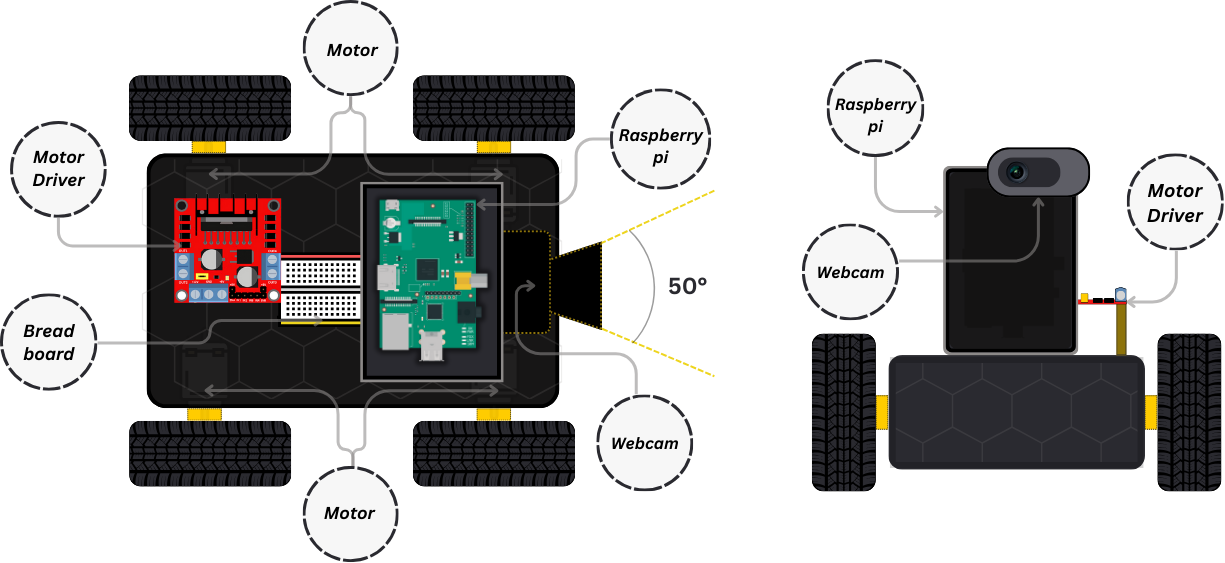
\includegraphics[width=1\textwidth]{ch4/figs/robot_car.png}
	\caption{Illustration of the hardware layout, showing the arrangement of key components like the Raspberry Pi, motor system, and camera module.}
	\label{fig:hardware_layout}
\end{figure}

The core decision-making process involved selecting the appropriate technologies and components. Based on the findings from previous research (e.g., Jacobsen et al. \cite{jacobsen2018}, La Delfa et al. \cite{delfa2015}, and Vanitha et al. \cite{vanitha2016}), which explored various mobile robot control methods using augmented reality (AR) and computer vision, it became clear that a Raspberry Pi-based system with a web interface would provide the required flexibility and ease of control for this project.

After evaluating several options for actuation and navigation, it was determined that motorized control through a motor driver and a four-wheel drive system would provide the most reliable and efficient solution for movement. This decision was supported by studies that demonstrate the performance of motor-driven robots in both laboratory and dynamic environments. Additionally, the use of fiducial markers, such as ArUco or AprilTag markers, was identified as a robust solution for localization and obstacle avoidance (La Delfa et al. \cite{delfa2015}; Vanitha et al. \cite{vanitha2016}).


\section{\label{sec:hardware} Hardware System Architecture}

The system architecture provides a high-level overview of how the robot and its subsystems interact with one another to achieve semi-autonomous navigation, real-time feedback, and remote control functionality. The key components of the system include the hardware modules such as the Raspberry Pi, motors, sensors, and camera, alongside software elements such as computer vision algorithms and the web-based control interface.

The project is composed of several key components, below is a high level overview of all the components that are needed in order execute the project properly.

\subsection{Micro-controller Selection}

The Raspberry Pi Model 4B with 4GB RAM was selected as the micro controller for this project due to its versatility and capability to handle multiple complex tasks simultaneously. Its ability to run sophisticated computer vision algorithms while interfacing with other hardware components makes it ideal for this application. The capacity to manage real-time video streaming, marker detection, and motor control simultaneously is crucial for the system's functionality.

Unlike dedicated micro-controllers(processors) such as the Arduino, the Raspberry Pi can run Python-based frameworks like OpenCV, which is essential for implementing the system's computer vision capabilities. This aligns with findings from Jacobsen et al. \cite{jacobsen2018}, who demonstrated the effectiveness of using a Raspberry Pi for web hosting.

The use of a single, integrated system for both processing and control, as highlighted in Chapter\ref{ch:lit_review}, simplifies the overall design, reduces latency, and enhances system performance. In our setup, the Raspberry Pi functions as the central processing unit, responsible for interfacing with all other components. It processes the video feed from the camera, executes computer vision algorithms such as ArUco marker detection, and transmits control signals to the motor driver. The Raspberry Pi runs a Python-based framework that integrates OpenCV for vision tasks and SocketIO for communication with the web interface. This allows it to receive input from the camera, process it using OpenCV, and then send commands to the motor driver based on the detected environment and user instructions received through the control interface.

The selection of the 4GB RAM version was made to ensure sufficient memory for running multiple processes concurrently and handling intensive computational tasks. While the 8GB version offers more memory, the 4GB model provides a balanced compromise between performance and cost-effectiveness for our application. Table \ref{table:pi_specs} provides a comparison of the specifications for the Raspberry Pi Model 4B with 4GB RAM:


\begin{table}[h!]
	\centering
	\begin{tabular}{|l|c|c|c|}
		\hline
		\textbf{Specification} & \textbf{2GB RAM} & \textbf{4GB RAM} & \textbf{8GB RAM} \\
		\hline
		\textbf{CPU} & Quad-core Cortex-A72 & Quad-core Cortex-A72 & Quad-core Cortex-A72 \\
		\hline
		\textbf{Clock Speed} & 1.5 GHz & 1.5 GHz & 1.5 GHz \\
		\hline
		\textbf{RAM} & 2GB LPDDR4 & 4GB LPDDR4 & 8GB LPDDR4 \\
		\hline
		\textbf{Networking} & Gigabit Ethernet & Gigabit Ethernet & Gigabit Ethernet \\
		\hline
		\textbf{USB Ports} & 2x USB 3.0, 2x USB 2.0 & 2x USB 3.0, 2x USB 2.0 & 2x USB 3.0, 2x USB 2.0 \\
		\hline
		\textbf{Video Output} & 2x micro-HDMI & 2x micro-HDMI & 2x micro-HDMI \\
		\hline
		\textbf{Power Supply} & 5V/3A USB-C & 5V/3A USB-C & 5V/3A USB-C \\
		\hline
	\end{tabular}
	\caption{Comparison of Raspberry Pi Model 4B RAM Versions}
	\label{table:pi_specs}
\end{table}

This hardware configuration provides the necessary processing power and memory to handle the computer vision tasks, video streaming, and robot control required by our project. The Raspberry Pi 4B with 4GB RAM offers a robust platform capable of running complex algorithms, processing real-time video data, and managing the various input and output operations essential for the robot car's operation.

\subsection{Camera Module}
The camera plays a pivotal role in this system as it provides real-time feedback necessary for detecting fiducial markers and controlling the robot's movement. The decision to use a high-resolution web camera, specifically the HD Logitech C270, over a more basic sensor was based on the need for precise marker detection, which demands high-quality image capture. La Delfa et al. \cite{delfa2015} emphasized the importance of high-resolution cameras for accurate marker detection, particularly in dynamic environments. A higher-quality video feed improves the reliability of computer vision algorithms and ensures better control over the robot’s movements.

The camera module continuously captures the video feed, which is streamed to both the user via the web interface and the Raspberry Pi for processing. The camera plays a critical role in detecting fiducial markers in the environment, enabling navigation and interaction based on visual feedback.

\begin{table}[h!]
	\centering
	\caption{Comparison of Logitech C270 and Raspberry Pi Camera Module V2}
	\begin{tabular}{|p{4cm}|p{5cm}|p{5cm}|}
		\hline
		\textbf{Specification}        & \textbf{Logitech C270}            & \textbf{Raspberry Pi Camera Module V2} \\ \hline
		\textbf{Resolution}           & 1280 x 720 (HD)                   & 3280 x 2464 (8 MP)                      \\ \hline
		\textbf{Frame Rate}           & 30 fps (at 720p)                  & 30 fps (at 1080p)                       \\ \hline
		\textbf{Field of View (FOV)}  & 60°                               & 62.2°                                   \\ \hline
		\textbf{Interface}            & USB                               & CSI (Camera Serial Interface)           \\ \hline
		\textbf{Price}                & Moderate                          & Low                                     \\ \hline
		\textbf{Ease of Use}          & Plug-and-play                     & Requires configuration                  \\ \hline
		\textbf{Compatibility}        & Universal (compatible with various systems) & Raspberry Pi exclusive                 \\ \hline
	\end{tabular}
	\label{tab:camera_comparison}
\end{table}


The Logitech C270 was chosen primarily due to it being readily available for use and its ability to seamlessly integrate into various systems via USB, requiring minimal configuration compared to the Raspberry Pi Camera Module. Additionally, while the Raspberry Pi camera offers higher resolution, the Logitech C270 provides sufficient image quality for marker detection. Furthermore, the webcam is universally compatible, making it a practical choice for prototyping and development in this context.


\subsection{Motor and Drive System}

The four-wheel drive system of the DGU ALUM MULTI-CHASSIS 4WD KIT was selected to ensure that the robot can move with precision across various terrains. This chassis provides a sturdy foundation for the robot's movement capabilities. The motors used in this system operate on 3V-12VDC, with a maximum torque of 800gf cm min at 4.5V. 

\section*{Motor Driver Selection}

To control the motors, a motor driver was necessary to interface with the Raspberry Pi and provide effective control over the speed and direction. Several motor driver options were considered before selecting the L298N H-bridge for its compatibility and ease of use. The alternatives explored included the DRV8833 and the TB6612FNG, each offering unique advantages. A comparison of these motor drivers is provided in Table \ref{tab:motor_driver_comparison}.

\begin{table}[h!]
	\centering
	\caption{Comparison of Motor Driver Options}
	\begin{tabular}{|p{3cm}|p{3cm}|p{3cm}|p{3cm}|}
		\hline
		\textbf{Specification}        & \textbf{L298N H-bridge} & \textbf{DRV8833}   & \textbf{TB6612FNG}   \\ \hline
		\textbf{Voltage Range}        & 5V - 46V                & 2.7V - 10.8V       & 4.5V - 13.5V         \\ \hline
		\textbf{Max Current}          & 2A per channel          & 1.5A per channel   & 1.2A per channel     \\ \hline
		\textbf{PWM Control}          & Yes                     & Yes                & Yes                  \\ \hline
		\textbf{Size}                 & Larger (bulky)          & Compact            & Compact              \\ \hline
		\textbf{Efficiency}           & Moderate (bipolar transistors) & High (MOSFETs)  & High (MOSFETs)       \\ \hline
		\textbf{Cost}                 & Low                     & Moderate           & Moderate             \\ \hline
	\end{tabular}
	\label{tab:motor_driver_comparison}
\end{table}

While the DRV8833 and TB6612FNG offer more compact designs and higher efficiency due to the use of MOSFETs, the L298N H-bridge was ultimately selected for this project. Its ability to handle higher voltage ranges and currents made it a better match for the motors in use. Additionally, the L298N supports straightforward Pulse Width Modulation (PWM) control, making it ideal for precise speed and direction control via the Raspberry Pi.


According to Vanitha et al. \cite{vanitha2016}, a robust motor and drive system is essential for mobile robots that rely on real-time feedback from sensors for navigation. The choice of using an H-bridge for motor control is well-supported in robotics literature as it allows for both forward and reverse motion, as well as turning, without adding unnecessary complexity. The four-wheel drive system enables the robot's movement and maneuvering, with the L298N motor driver controlling the speed and direction of the motors based on the PWM signals received from the Raspberry Pi. This setup allows the system to adjust motor power dynamically to maintain proper navigation based on sensor input or user commands, achieving precise movement in various scenarios.

\begin{figure}[H]
	\centering

		\centering
		\includegraphics[width=0.835\textwidth]{ch4/figs/H-Bridge-Interface.png}
		\caption{Illustration of the H-Bridge connection with the motors.}
		\label{fig:motor_H-bridge_connection}
	\end{figure}


\begin{table}[h]
	\centering
	\begin{tabular}{|c|c|c|c|c|c|c|}
		\hline
		\textbf{IN1} & \textbf{IN2} & \textbf{IN3} & \textbf{IN4} & \textbf{Motor A/B} & \textbf{Motor C/D} & \textbf{Robot Movement} \\
		\hline
		0 & 1 & 0 & 1 & Forward & Forward & Forward \\
		\hline
		1 & 0 & 1 & 0 & Reverse & Reverse & Reverse \\
		\hline
		0 & 1 & 1 & 0 & Forward & Reverse & Right Turn \\
		\hline
		1 & 0 & 0 & 1 & Reverse & Forward & Left Turn \\
		\hline
		0 & 0 & 0 & 0 & Stop & Stop & Stop \\
		\hline
		1 & 1 & 1 & 1 & Brake & Brake & Brake \\
		\hline
	\end{tabular}
	\caption{Truth Table for L298N H-Bridge Motor Control}
	\label{tab:condensed_hbridge_control}
\end{table}

The Raspberry Pi generates PWM (Pulse Width Modulation) signals through its GPIO pins, which are connected to the input pins (IN1, IN2, IN3, IN4) of the L298N H-bridge motor driver. These digital signals control the direction and speed of the motors. The H-bridge then interprets these signals and converts them into the appropriate voltage levels and current flow to drive the motors. For Motors A and B, IN1 and IN2 control their direction and speed, while IN3 and IN4 control Motors C and D. The H-bridge acts as an intermediary, amplifying the low-power signals from the Raspberry Pi into the higher power (by using an external power source) needed to drive the DC motors effectively. This setup allows for precise control over each motor's behavior, enabling complex movements of the robot through simple digital commands from the Raspberry Pi.

\section{Power Supply}

Although the primary focus of this project is the robot's navigation, control systems, and augmented reality (AR) integration, the power supply plays a vital role in ensuring reliable performance for the entire system. Without a stable and appropriate power source, the Raspberry Pi, motors, and other components would fail to operate consistently, which could result in unpredictable robot behavior. To address the varying power needs of the system components, two separate power supplies were implemented.

\subsection{Raspberry Pi Power Supply}
The Raspberry Pi requires a consistent and stable power supply to handle its computational tasks, including image processing, web-based control, and communication with other subsystems. A power bank was selected for this purpose due to its wide availability, ease of use, and sufficient power output.

\begin{itemize}
	\item \textbf{Power Source:} A commercial power bank with a 2.1A output was utilized to meet the power requirements of the Raspberry Pi 4.
	
	\item \textbf{Reason for Choice:} The Raspberry Pi 4 requires a power supply that can provide at least \textbf{5V and 3A} for optimal performance. While the chosen power bank offers slightly lower current (2.1A), testing showed that it was sufficient for running the robot's tasks without significant performance degradation. Additionally, the portability and long-lasting capacity of the power bank make it ideal for mobile robotics applications.
	
\end{itemize}

\subsection{H-Bridge and Motor Power Supply}
The L298N H-bridge motor driver and the motors require a different power supply than the Raspberry Pi, given their higher power demands during operation, particularly under load (e.g., when turning or climbing). To meet this requirement, an RS PRO 3C 3S1P Li-Ion Battery Pack was chosen, which offers higher voltage and capacity.


The battery pack consists of \textbf{three 18650 Li-Ion cells} connected in series (3S1P configuration), providing a total voltage of \textbf{11.1V} and a capacity of \textbf{2600mAh}.
	
\textbf{Specifications:}
	\begin{itemize}
		\item Voltage: 11.1V
		\item Capacity: 2600mAh
		\item Configuration: 3 x 18650 cells in series
	\end{itemize}
	
\textbf{Reason for Choice:} The L298N H-bridge can handle up to 46V, so 11.1V is well within its operational range. The motors benefit from higher voltage when performing tasks that require more torque, such as sharp turns or accelerating from a stationary position. The 2600mAh capacity ensures that the robot can operate for extended periods before needing a recharge.
	

\section{\label{sec:software} Software System Architecture}

The bulk of the project relied on software for functionality, serving as the brain of the entire system. The software orchestrates communication between hardware components and enables real-time decision-making. This architecture integrates several critical subsystems, including computer vision, motor control, data processing, and network communication.

Python was chosen as the primary programming language for the project, largely due to its versatility and the wide range of libraries it offers, particularly in fields like robotics, image processing (OpenCV), and web development (Flask). Although other programming languages such as C++ or Java were considered, Python stood out because of its simplicity, ease of development, and extensive library support, the timeline of the project also did not allow for use of a lower level language like C. These qualities made it an ideal choice for rapid prototyping and achieving the project’s deliverables within the given time constraints.


\begin{figure}[H]
	\centering
	
	\centering
	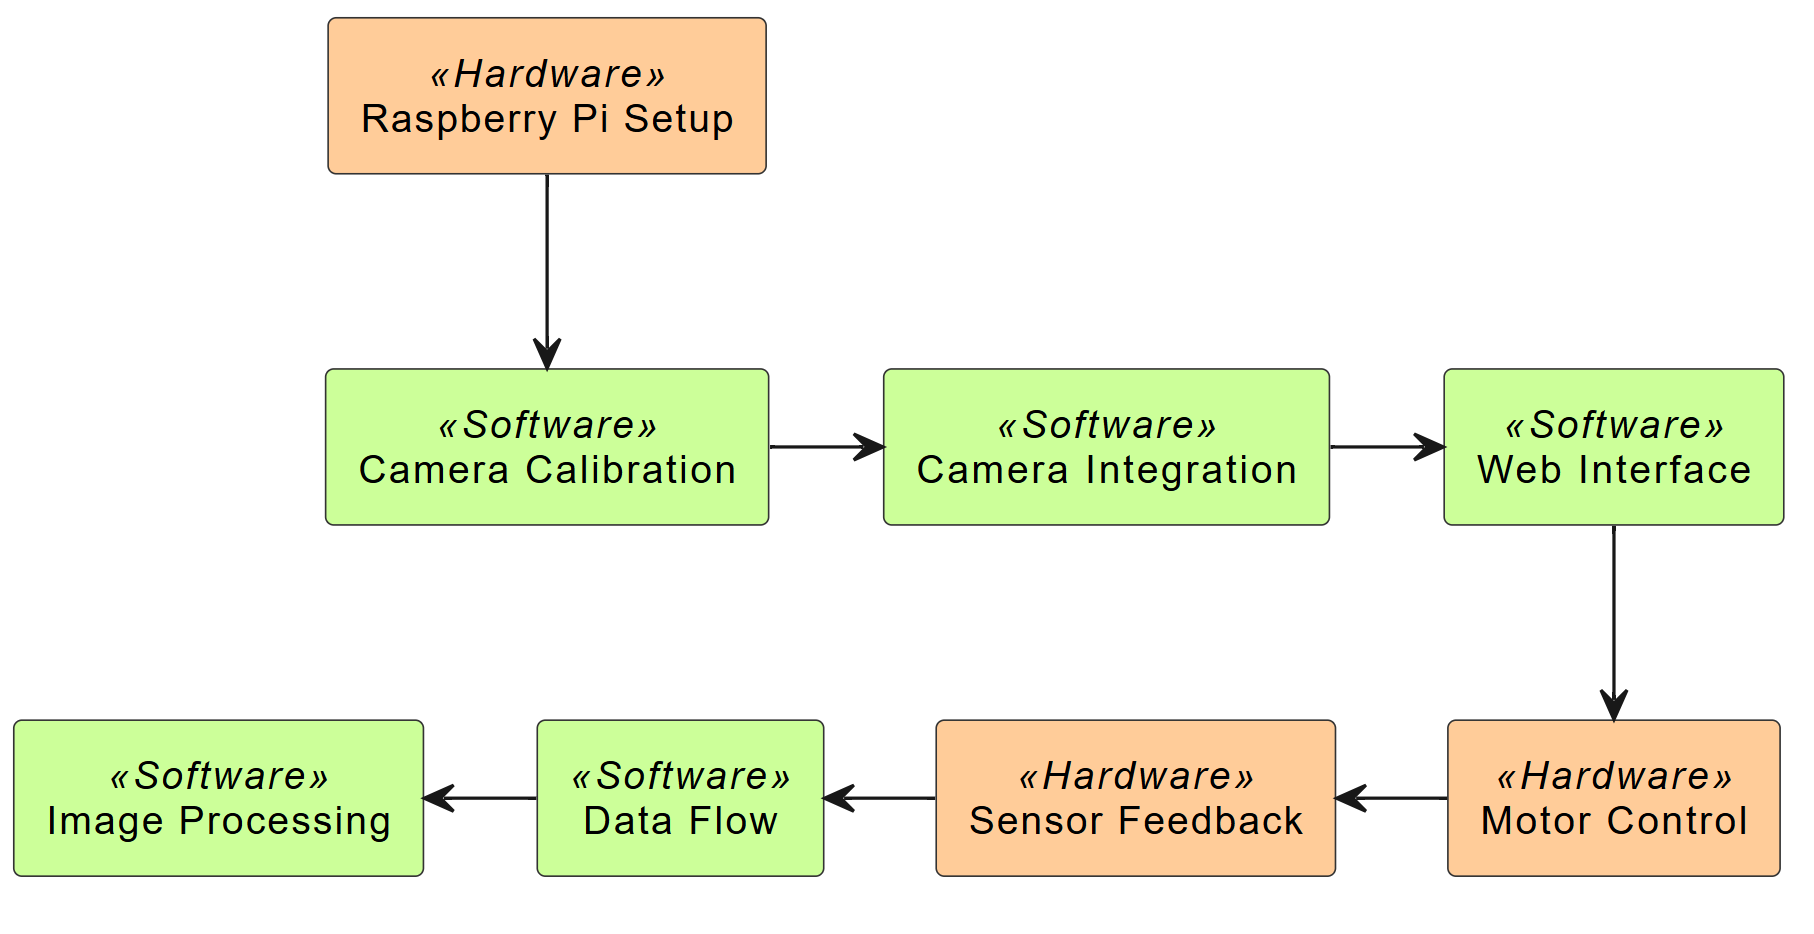
\includegraphics[width=0.8\textwidth]{ch4/figs/hi.png}
	\caption{Illustration of the project production process.}
	\label{fig:process}
\end{figure}

Figure \ref{fig:process} provides an overview of the project production process. The flow begins with setting up the software environment on the Raspberry Pi, followed by camera calibration and integration, which is crucial for enabling accurate image capture and processing. These steps lead to the development of a web interface, facilitating interaction with the system. The software is then responsible for managing data flow between image processing algorithms and sensor feedback, which in turn, directly informs motor control to achieve desired movements and responses. Below I delve into the design of each system.

\subsection{Development Environment Setup}

To begin the development of the robot, I set up a headless Raspberry Pi environment, which means that I connected to the Pi remotely over SSH, avoiding the need for a physical monitor, keyboard, or mouse. This headless setup is common for Raspberry Pi projects where the Pi is used as an embedded device, and allows for easier control via the network from my laptop. I initiated an SSH session using the command:

\begin{quote}
	\texttt{ssh pi@<raspberry-pi-ip>}
\end{quote}

from my development machine to connect to the Pi and began the process of setting up the environment.

The primary goal of the development environment was to create a clean, isolated workspace that would avoid interfering with the Pi’s system libraries and default configurations. To achieve this, I decided to set up a virtual Python environment using \texttt{venv}, which would ensure that all libraries required for this project were contained within the environment and did not alter the system’s default Python packages.

To create and activate the environment, I ran:

\begin{quote}
	\texttt{python3 -m venv robot\_env} \\
	\texttt{source robot\_env/bin/activate}
\end{quote}

The project depended on several libraries for various functions. Some of these libraries were for The project depended on several libraries for various functions. Some of these libraries were for \textbf{web development}, like \textbf{Flask} and \textbf{Flask-SocketIO}, which handled real-time communication between the Raspberry Pi and the web interface. Others were for \textbf{computer vision}, including \textbf{OpenCV} and \textbf{ArUco}, which would handle marker detection and processing of the video feed.


To install the required libraries, I used \texttt{pip} within the activated virtual environment. Here is the command that I used to install all the necessary dependencies Each of these libraries served a specific purpose:

\begin{table}[H]
	\centering
	\begin{tabular}{|p{3cm}|p{12cm}|}
		\hline
		\textbf{Library/Tool} & \textbf{Description} \\ 
		\hline
		\textbf{Flask} & Creates the web server for video streaming and control commands. \\ 
		\hline
		\textbf{Flask-SocketIO} & Enables real-time communication for responsive robot control. \\ 
		\hline
		\textbf{OpenCV} & Handles video capture and ArUco marker detection for navigation. \\ 
		\hline
		\textbf{aiortc} & Supports WebRTC for live video streaming from the robot's camera. \\ 
		\hline
		\textbf{pigpio} & Controls GPIO pins with high precision for better timing. \\ 
		\hline
		\textbf{Numpy} & Manages arrays and matrix operations for image processing. \\ 
		\hline
		\textbf{uuid} \& \textbf{asyncio} & Generates unique IDs and manages asynchronous operations for WebRTC. \\ 
		\hline
	\end{tabular}
	\caption{Summary of libraries and tools used in the project.}
	\label{tab:libs}
\end{table}



These libraries were specifically selected to ensure smooth operation of the robot’s core functions, including image processing, real-time control, and web interaction. 

\subsection{Camera Calibration}

Before proceeding with the implementation of the robot’s image processing pipeline, I first verified that the camera was functioning correctly. This involved ensuring that the Raspberry Pi camera module was properly connected and that the Raspberry Pi could capture live video feeds. Once this basic functionality was confirmed, the next step was to calibrate the camera to account for lens distortion, a crucial step for ensuring accurate marker detection later in the project.

To perform the calibration, I ran a \textbf{Flask web application} that captured and stored images from the camera for the calibration process. The process of camera calibration involves capturing multiple images of a checkerboard pattern at various angles, which allows for the correction of geometric distortions such as barrel distortion in the captured images. Using the images, I applied OpenCV’s camera calibration functionality to compute the intrinsic and distortion parameters of the camera.

The Flask app was set up to continuously stream the live feed from the camera and save frames at regular intervals. Below is a brief overview of the code used to capture images from the camera and store them for calibration:

\begin{figure}[H]
	\centering
	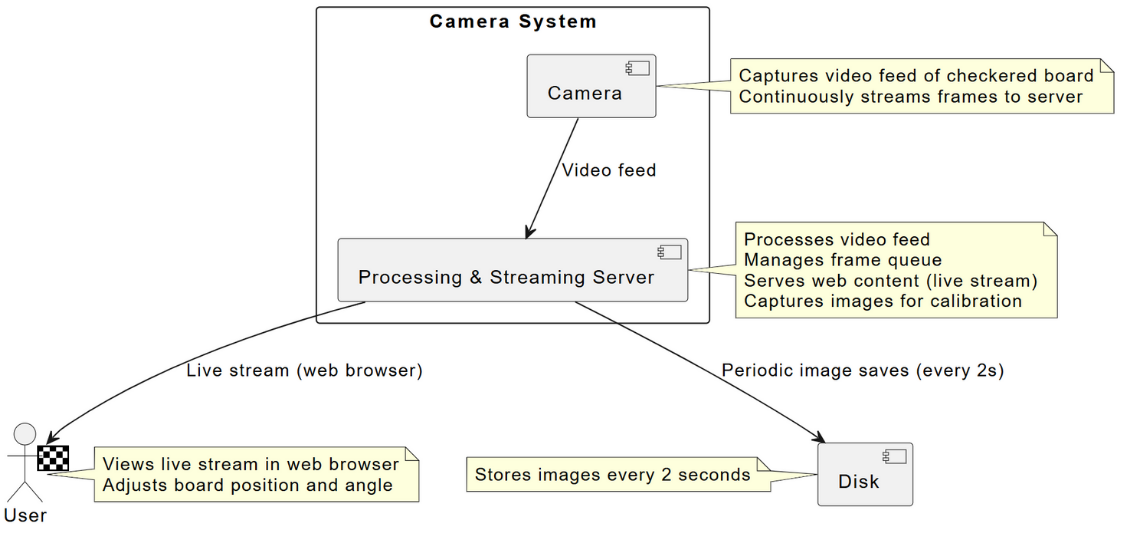
\includegraphics[width=0.9\textwidth]{ch4/figs/calibration.png}
	\caption{Diagram of the functionality of the calibration app.}
	\label{fig:calibration}
\end{figure}

After confirming the camera’s functionality, I captured a series of images through the Flask app, which were then processed using OpenCV’s camera calibration tools. The calibration process computes the intrinsic camera matrix and distortion coefficients, which are essential for removing distortion and ensuring the accuracy of subsequent image processing steps.

OpenCV's camera calibration tool was used, with images of a checkerboard pattern captured by the camera. The following steps were followed for the calibration:

\begin{enumerate}
	\item \textbf{Capture Images}: The Flask app automatically saved images at a regular interval during the video feed, stored in the specified directory.
	\item \textbf{Camera Calibration}: Using OpenCV, the captured images were processed to detect the checkerboard pattern and calculate the camera’s intrinsic and distortion parameters.
	\item \textbf{Saving Results}: Once the camera was successfully calibrated, the calibration parameters (including the camera matrix and distortion coefficients) were saved to a YAML file, which could be used later for distortion correction in real-time video processing.
\end{enumerate}

The resulting calibration file was stored in calibration.yaml, which contained the necessary parameters for correcting lens distortion during subsequent image processing tasks. This YAML file is crucial for ensuring that the robot can accurately interpret the positions of ArUco markers in real-world coordinates, even when captured through distorted lenses.


\subsection{ArUco Marker Detection}

The implementation of ArUco markers in this project leverages their speed and reliability, crucial for real-time robotics applications. ArUco outperforms alternatives like AprilTag and CCTag, with detection times as low as 2 milliseconds on minimalist hardware setups \cite{patru2023empirical}. This efficiency is vital for our Raspberry Pi-based mobile robot system, where rapid visual data interpretation ensures smooth navigation and environmental interaction.

Beyond basic detection, ArUco markers enable advanced features such as distance measurement and speed estimation. The system utilizes the known marker size and camera frame appearance to estimate robot-to-marker distance, forming the basis for speed calculations.

\subsubsection{Distance Measurement}

Distance measurement is implemented using the \texttt{estimate\_pose} function:

\begin{verbatim}
	distance = self.estimate_pose(corners)
\end{verbatim}

This function uses the marker's known physical size and camera intrinsic parameters to estimate the marker's pose relative to the camera. The distance \(d\) is then calculated using the translation vector \(\mathbf{t}\) from the pose estimation:

\[
d = \|\mathbf{t}\| = \sqrt{t_x^2 + t_y^2 + t_z^2}
\]

\subsubsection{Speed Estimation}

Speed estimation employs a rolling buffer approach for stable readings. The implementation of a buffer-based speed calculation method, as opposed to a simpler instantaneous approach, was chosen to enhance the robustness and reliability of the system's speed estimates. While a basic speed calculation using only the most recent two data points ($v = \frac{\Delta d}{\Delta t}$) would be computationally simpler, it would be highly susceptible to noise and momentary fluctuations in distance measurements or marker detection. Our buffer-based method, which maintains a rolling window of recent measurements, allows for a more stable and accurate speed estimation by averaging over multiple data points. 

The speed calculation occurs in the \texttt{calculate\_speed} method:

\begin{verbatim}
	def calculate_speed(self, current_distance, current_time):
\end{verbatim}

The instantaneous speed \(v_i\) between two consecutive measurements is calculated as:

\[
v_i = \left|\frac{\Delta d_i}{\Delta t_i}\right| = \left|\frac{d_i - d_{i-1}}{t_i - t_{i-1}}\right|
\]

where \(d_i\) and \(t_i\) are the distance and time at the \(i\)-th measurement, respectively.

The average speed \(\bar{v}\) over the buffer is then computed as:

\[
\bar{v} = \frac{1}{n} \sum_{i=1}^{n} v_i
\]

where \(n\) is the number of valid speed measurements in the buffer.


The integration of ArUco markers with these distance and speed estimation techniques enables the creation of control zones and the overlay of augmented reality (AR) elements. For instance, upon detecting a "restricted zone" marker, the robot can dynamically adjust its speed or trajectory based on the calculated distance and speed.

The analysis in \cite{patru2023empirical} emphasizes ArUco's superior performance in speed-dependent tasks, which is crucial for our application where the robot must accurately detect and interpret markers while in motion, facilitating real-time distance and speed calculations.

Given the computational constraints of the Raspberry Pi, the efficiency of the ArUco algorithm, combined with our optimized distance and speed estimation techniques, proves ideal for this project. This setup ensures real-time performance and reliable detection, allowing the robot to respond dynamically to environmental changes based on detected markers and calculated metrics.


\subsection{Obstacle Detection System}

The obstacle detection system in this project utilizes the YOLOv5n (You Only Look Once, version 5 nano) model, a lightweight and efficient neural network designed for real-time object detection. YOLOv5n's compact size and low computational requirements make it ideal for embedded applications like our mobile robot, enabling fast inference on devices with limited processing power such as the Raspberry Pi.

\subsubsection{Model Configuration}

The YOLOv5n model is configured specifically for our use case:

\begin{lstlisting}[style=pythonstyle, caption=YOLOv5n cofiguration]
	def setup_yolo_model(self):
	self.model = torch.hub.load('ultralytics/yolov5', 'yolov5n', pretrained=True)
	self.model.classes = [39]  # Class 39 for bottle detection
	self.model.conf = 0.1  # Confidence threshold
	self.model.iou = 0.45  # IOU threshold for NMS
	self.model.to('cpu')  # Ensure CPU execution
\end{lstlisting}

This configuration focuses on detecting a single class of objects (bottles, class 39) to optimize processing power and speed. The confidence threshold (\texttt{conf}) is set to 0.1, striking a balance between detection sensitivity and false positive reduction. The Intersection over Union (IoU) threshold for non-maximum suppression is set to 0.45, helping to eliminate redundant detections.

\subsubsection{Detection Process}

The obstacle detection process is implemented in the \texttt{detect\_obstacles} method:

\begin{lstlisting}[style=pythonstyle, caption=YOLOv5n detection Process]
	def detect_obstacles(self, frame):
	results = self.model(frame)
	self.obstacle_detected = False
	for *xyxy, conf, cls in results.xyxy[0]:
	if conf > self.model.conf:
	# Obstacle detected, mark frame and set flag
\end{lstlisting}

This method processes each frame through the YOLO model and checks for detections above the confidence threshold. When an obstacle (bottle) is detected, it's marked on the frame and a flag is set.

Notably, the obstacle detection is not continuously active. It's designed to be user-activated via the control interface, optimizing power consumption and reducing potential latency in the video feed. When activated, it processes frames in real-time, providing immediate feedback to the control system if an obstacle is detected.

\subsubsection{Performance Considerations}

The decision to detect only a single object class (bottles) significantly reduces the computational load compared to multi-class detection. This approach is justified by the specific use case of our robot and the need to balance detection capabilities with real-time performance on limited hardware.

The performance of this system can be characterized by its inference time $t_i$, which is the time taken to process a single frame:

\[
t_i = t_p + t_d + t_m
\]

Where:
\begin{itemize}
	\item $t_p$ is the preprocessing time (frame acquisition and conversion)
	\item $t_d$ is the YOLO model inference time
	\item $t_m$ is the post-processing time (drawing bounding boxes, updating flags)
\end{itemize}

By focusing on a single class and using the lightweight YOLOv5n model, we minimize $t_d$, which is typically the most significant component of $t_i$.

This design balances detection capabilities with resource efficiency, making the obstacle detection system both responsive and power-conscious. It allows the robot to operate normally under default conditions and only initiates the obstacle detection process when necessary, providing a flexible and efficient solution for real-time obstacle avoidance in mobile robotics applications.

\subsection{Wheel Interface Design}

The wheel interface was designed to control four motors, arranged in pairs, connected to an L298N H-bridge motor driver. Each pair of motors is responsible for controlling the left and right sides of the robot, allowing for differential steering. The system uses the Raspberry Pi's GPIO pins to control the direction and speed of the motors through Pulse Width Modulation (PWM).

\subsubsection{Motor Control Using GPIO and PWM}

Each motor pair is controlled using two GPIO pins for direction control and one PWM pin for speed control. The L298N H-bridge allows the Raspberry Pi to control the motors in both forward and reverse directions by manipulating the GPIO pins. The PWM signal controls the speed of the motors by adjusting the duty cycle of the signal sent to the H-bridge.

\begin{itemize}
	\item \textbf{Forward Movement}: Both pairs of motors are driven in the same direction, with a high signal sent to the forward GPIO pin and a low signal to the reverse pin. The PWM signal controls the speed of both motor pairs, allowing the robot to move forward.
	\item \textbf{Turning}: To turn, the speed or direction of one pair of motors is adjusted. For example, to turn left, the left motor pair is reversed, while the right motor pair continues to move forward.
	\item \textbf{Stop}: The robot is stopped by setting all GPIO pins to low, cutting off the power to both motor pairs.
\end{itemize}

\subsubsection{Integration with Web Interface}

The web interface allows the user to control the robot in real-time by sending movement commands via Flask-SocketIO. These commands are mapped to motor control functions in the backend, where the GPIO pins are set according to the desired direction and speed. The key inputs (W, A, S, D) correspond to forward, left, backward, and right movements, which are translated into GPIO signals for the motor pairs.

\begin{itemize}
	\item \textbf{W Key}: Moves the robot forward by setting both motor pairs to move in the forward direction.
	\item \textbf{S Key}: Reverses both motor pairs to move the robot backward.
	\item \textbf{A Key}: Adjusts the motor speed and direction to turn left by slowing down or reversing the left motor pair.
	\item \textbf{D Key}: Adjusts the motor speed and direction to turn right by slowing down or reversing the right motor pair.
\end{itemize}

This design provides precise control over the robot’s movements and allows the user to navigate the robot using the web interface in real-time. By using PWM, the robot’s speed can be smoothly adjusted based on the user’s input.

\subsection{Web Interface and Server Design}
The web interface and server design are crucial components of this project, enabling remote control and real-time monitoring of the robot's movements. The system was designed to create a lightweight and responsive interface accessible through a standard web browser, allowing users to control the robot and view live feedback from the camera in real-time.

\subsubsection{Server Architecture}
The server was built using the Flask framework, a micro web framework for Python, chosen for its simplicity and efficiency in handling web requests, streaming video data, and managing control inputs from the user.

The core architecture of the server includes the following key components:
\begin{itemize}
	\item \textbf{Flask Web Server}: Responsible for serving the main web page and handling HTTP requests. Flask's flexibility allows for seamless integration of both static files (HTML, JavaScript, CSS) and dynamic content (video streaming).
	\item \textbf{SocketIO Integration}: Flask-SocketIO was implemented for real-time, bidirectional communication between the web interface and the robot. This allows the web client to send control commands to the robot without page reloads and enables real-time feedback by pushing updates to the client.
	\item \textbf{Video Streaming}: The robot's camera feed is streamed to the web interface using Flask's response streaming mechanism. Video frames are captured, processed, and sent to the web client for near real-time display.
	\item \textbf{WebRTC Integration}: For improved video streaming performance, WebRTC (Web Real-Time Communication) was implemented using the aiortc library, allowing for peer-to-peer video transmission.
\end{itemize}

\subsubsection{Web Interface Design}
The web interface was designed to be intuitive and responsive, built using HTML5, CSS, and JavaScript. It allows users to control the robot through both on-screen buttons and keyboard inputs.

\begin{figure}[H]
	\centering
	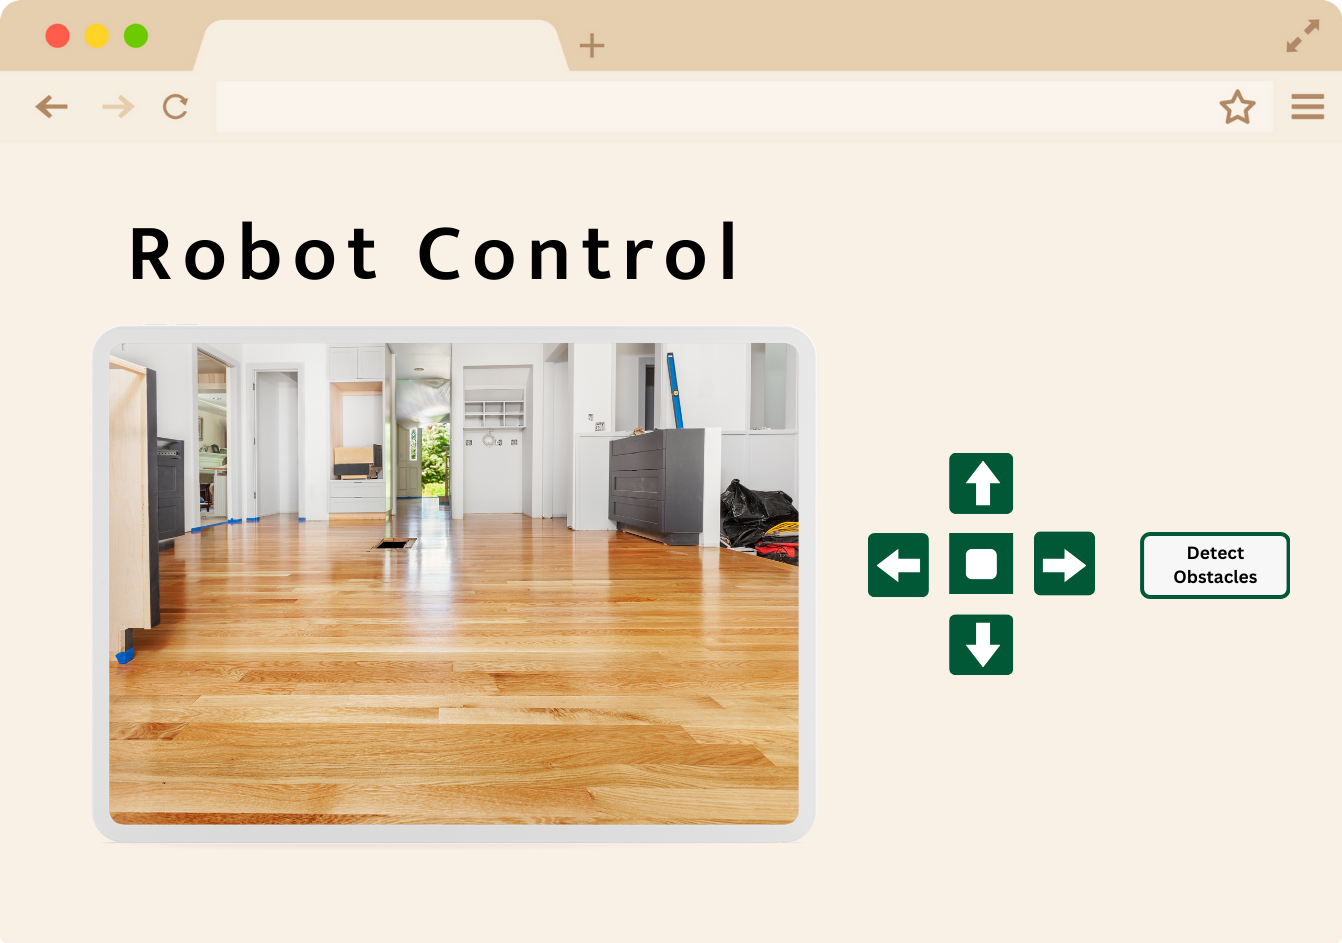
\includegraphics[width=0.7\linewidth]{ch4/figs/website}
	\caption{Visualization of front-end client side server}
	\label{fig:website}
\end{figure}

Key features of the web interface include:
\begin{itemize}
	\item \textbf{Control Panel}: A set of virtual buttons for controlling the robot's movements (forward, backward, left, right, stop). These controls are mapped to the robot's movement functions through SocketIO.
	\item \textbf{Live Video Feed}: An embedded video player streams the live feed from the robot's camera, allowing users to see the robot's perspective in real-time.
	\item \textbf{Keyboard Control}: Users can control the robot using keyboard inputs (W, A, S, D keys and arrow keys), providing an alternative to on-screen buttons.
	\item \textbf{Bottle Detection Toggle}: A button to enable or disable the bottle detection feature, demonstrating the system's capability for object recognition.
\end{itemize}

\subsubsection{Server-Side Implementation}
The server-side implementation includes several key functions in a sleek minimalist layout:

\begin{itemize}
	\item \textbf{Route Setup}: Flask routes are defined for serving the main page ('/') and the video feed ('/video\_feed').
	\item \textbf{Movement Handling}: SocketIO events handle movement commands, translating them into appropriate robot actions. This includes a safety feature to disable forward movement when a restricted zone is detected.
	\item \textbf{Bottle Detection Toggle}: A SocketIO event handler toggles the bottle detection feature on and off based on user input.
	\item \textbf{WebRTC Offer Handling}: An asynchronous function handles WebRTC offers, setting up peer connections for improved video streaming.
	\item \textbf{UI Interaction Handling}: SocketIO events process user interface interactions, allowing for real-time updates and feedback.
\end{itemize}

\subsubsection{Design Considerations}
\textbf{Performance and Latency}: Real-time operation necessitated minimizing latency in both video streaming and control inputs. The use of SocketIO for control commands and WebRTC for video streaming helps achieve low-latency communication. The video stream is optimized using a lower resolution and frame rate to reduce the load on the Raspberry Pi and ensure smoother performance.

\textbf{Responsive Design}: The interface is designed to be responsive, adapting to different screen sizes and devices. This ensures a consistent user experience across desktop and mobile browsers.

\textbf{Modularity}: The server architecture is designed with modularity in mind, separating concerns between route handling, video processing, and robot control. This design facilitates easier maintenance and potential future expansions of the system.

\subsubsection{Testing and Validation}
To ensure the reliability and performance of the web interface and server, a series of tests were conducted:

\begin{itemize}
	\item \textbf{Functional Testing}: Each control and feature of the web interface was tested to ensure correct operation.
	\item \textbf{Latency Testing}: The responsiveness of robot controls and video feed was measured to ensure acceptable real-time performance.
	\item \textbf{Cross-browser Testing}: The interface was tested across multiple browsers to ensure compatibility.
	\item \textbf{Mobile Responsiveness Testing}: The interface was tested on various mobile devices to verify its responsive design.
\end{itemize}

These tests helped refine the design and improve the overall user experience of the web interface and server components. For more details into how these tests were run and the results generated refer to the following chapter.